\documentclass[a4paper,10pt]{article}
\usepackage[utf8]{inputenc}

\usepackage{amsmath}
\usepackage{amssymb}
\usepackage[left=2cm,right=2cm,top=2cm,bottom=2cm]{geometry}
\usepackage{graphicx}
\usepackage{epstopdf}
\usepackage[compact]{titlesec}

%opening
\title{Hall term 2nd order correction terms in the field solver's Ohm's law}
\author{Yann Kempf}
\date{\today}

\newcommand{\E}{\mathbf{E}}
\newcommand{\B}{\mathbf{B}}
\newcommand{\Be}{\mathbf{B}^\mathrm{E}}
\newcommand{\Bex}{B^{\mathrm{E}x}}
\newcommand{\Bey}{B^{\mathrm{E}y}}
\newcommand{\Bez}{B^{\mathrm{E}z}}
\newcommand{\avBe}{\bar{\mathbf{B}}^\mathrm{E}}
\newcommand{\avBex}{\bar{B}^{\mathrm{E}x}}
\newcommand{\avBey}{\bar{B}^{\mathrm{E}y}}
\newcommand{\avBez}{\bar{B}^{\mathrm{E}z}}
\newcommand{\Bf}{\mathbf{B}^{\mathrm{F}}}
\newcommand{\Bfx}{B^{\mathrm{F}x}}
\newcommand{\Bfy}{B^{\mathrm{F}y}}
\newcommand{\Bfz}{B^{\mathrm{F}z}}
\newcommand{\J}{\mathbf{j}}
\newcommand{\pp}[1]{\left(#1\right)}
\newcommand{\DX}{\Delta X}
\newcommand{\DY}{\Delta Y}
\newcommand{\DZ}{\Delta Z}

\begin{document}

\maketitle

\begin{abstract}
For review and reference I want to list here the derivation of the correction
terms for the Hall term in Ohm's law in the field solver.
\end{abstract}

\section{Variables and principle}
The Londrillo \& Del Zanna field solver propagates the electric field $\E$
components averaged over a simulation cell's edges and the magnetic field $\B$
components averaged over a cell's faces. See Figure \ref{fig:Components} for a
schematic view.

The electric field averaged along the cell's edges is computed using Ohm's law
\begin{equation}
   \E = -\mathbf{V}\times\B + \frac{1}{\rho_q}\J\times\B.
\end{equation}
The second-order accuracy of the ideal part $\E=-\mathbf{V}\times\B$ is dealt
with by the field solver. For the Hall term we need to add correction terms to
ensure the second-order accuracy as neither $\J$ nor $\B$ are located on the
cell edges.

The plan is:
\begin{enumerate}
   \item Compute $\Be$ averaged on the edges starting from the face-averaged
values $\Bf$ with interpolations up to second derivatives in order to recover
the correct order when taking the components' first derivatives.
   \item Compute $\J=\nabla\times\Be/\mu_0$ on the edge.
   \item Compute the Hall term $\J\times\Be$ for Ohm's law using both $\J$ and
$\Be$ which are located on the cell edges.
\end{enumerate}

For this we need (new features in the code) to:
\begin{itemize}
   \item Compute all second derivatives of $\Bf$ in order to interpolate to
get the $\Be$ properly;
   \begin{itemize}
      \item Thus we need an extended stencil and possibly different schemes at
boundaries;
   \end{itemize}
   \item Calculate $\Be$;
   \item Communicate $\Be$;
   \item Calculate $\J$ using $\Be$;
   \item Calculate $\J\times\Be$ in Ohm's law with the new $\J$ and $\Be$.
\end{itemize}

The rest of this document handles some of these aspects in detail.


\begin{figure}
   \centering
   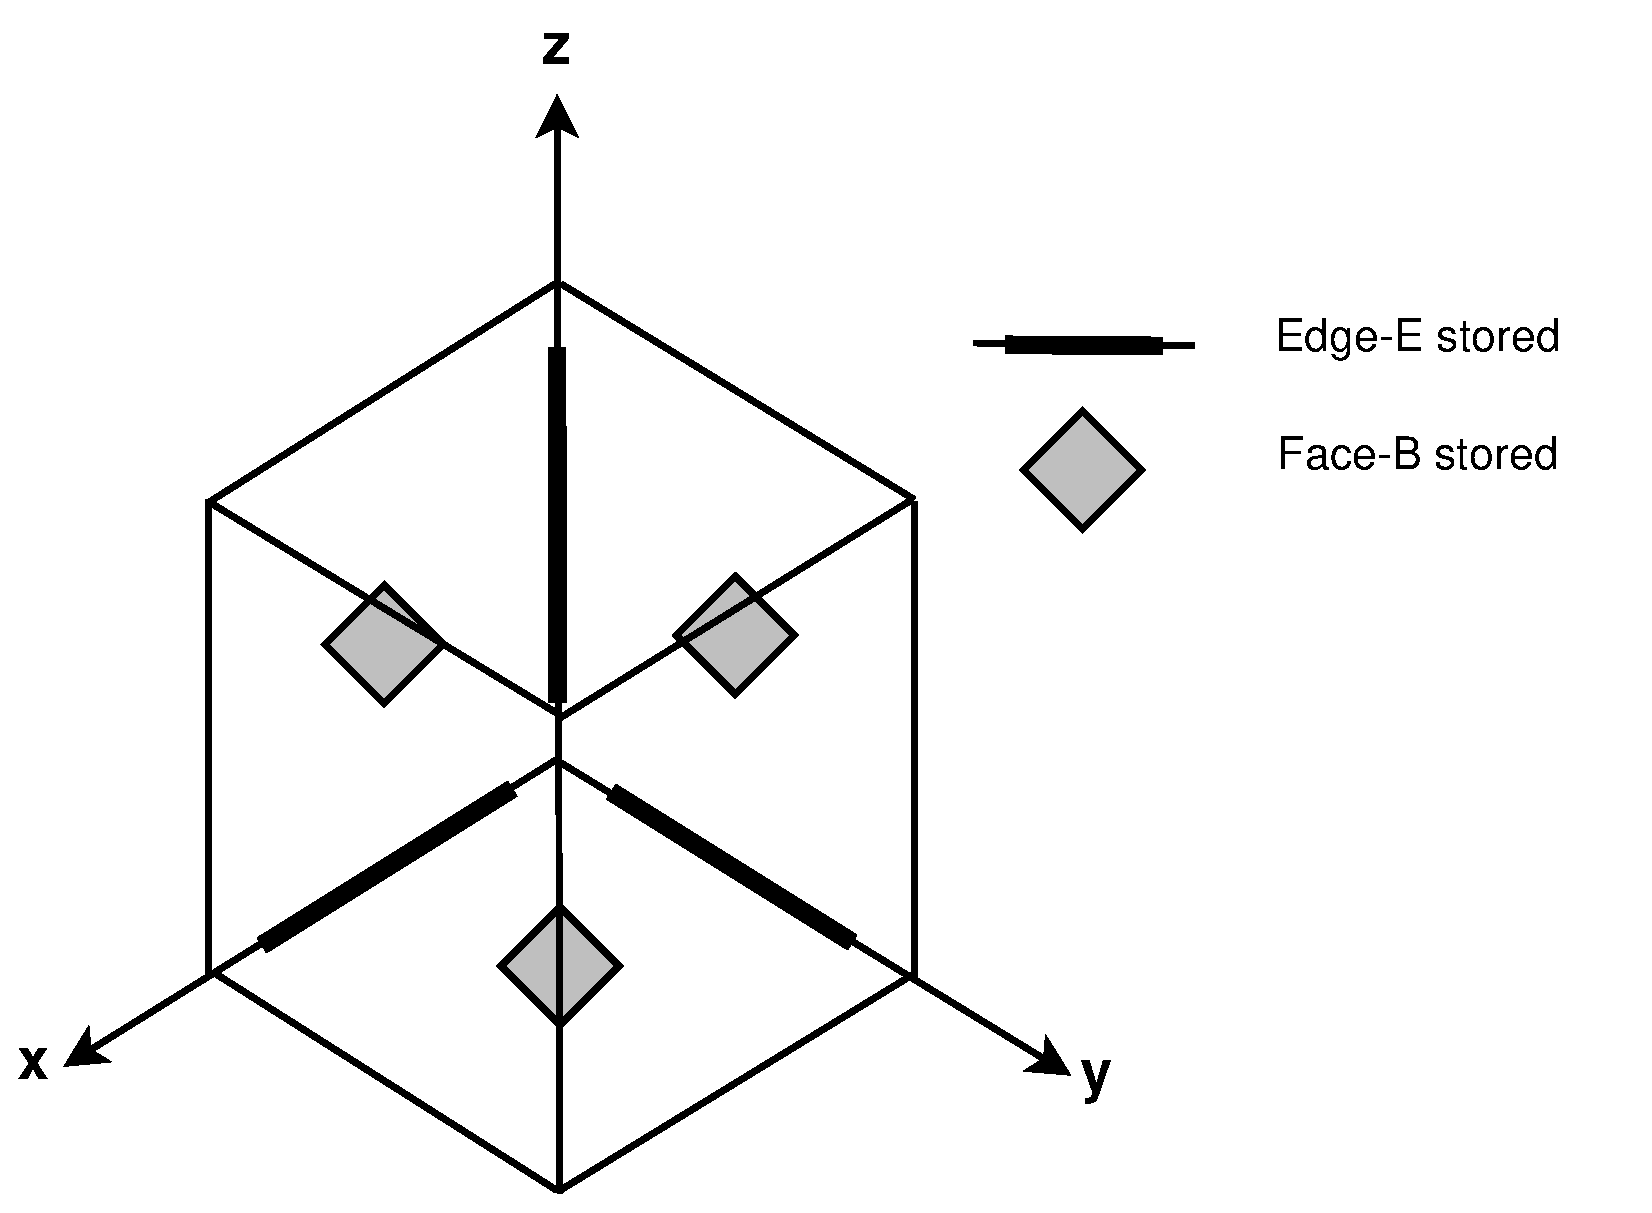
\includegraphics[width=0.5\textwidth]{variables.eps}
   \caption{Location of the $\E$ and $\B$ components in a spatial cell for the
field solver.}
\label{fig:Components}
\end{figure}




\section{Interpolation of $\Bf$ to $\Be$ up to second order derivatives}
In order for $\J$ to be of the right order, being computed as derivatives of
$\Be$, $\Be$ must be interpolated from $\Bf$ using first- and second-order
derivatives (Taylor expansion). The nomenclature used here is:
\begin{description}
   \item[$^\mathrm{E}$] edge averaged;
   \item[$^\mathrm{F}$] face average;
   \item[$^\mathrm{En}$] edge averaged along edge $n$;
   \item[$^\mathrm{Fn}$] face averaged on face $n$;
   \item[$_n$] component n;
   \item[$_{,n}$] derivative along direction $n$;
   \item[$x,y,z$] coordinates in the cell;
   \item[$\Delta N$] cell size along $N$.
\end{description}
The coordinate system used has its origin at the centre of the cell, hence
faces $n$ are at coordinates $\pm\Delta n$.

\subsection{$\Be$ along the edges}
\begin{align}
\Bex_x = &\Bfx_x \nonumber
\\ &+
\Bfx_{x,x}\pp{x + \frac{\DX}{2}} -
\frac{1}{2}\Bfx_{x,y}\DY -
\frac{1}{2}\Bfx_{x,z}\DZ \nonumber
\\ &+
\frac{1}{2}\Bfx_{x,xx}\pp{x+\frac{\DX}{2}}^2 +
\frac{1}{8}\Bfx_{x,yy}\DY^2 +
\frac{1}{8}\Bfx_{x,zz}\DZ^2 \nonumber
\\ &-
\frac{1}{2}\Bfx_{x,xy}\DY\pp{x + \frac{\DX}{2}} +
\frac{1}{4}\Bfx_{x,yz}\DY\DZ -
\frac{1}{2}\Bfx_{x,zx}\DZ\pp{x + \frac{\DX}{2}}
%\end{align}
\\
%\begin{align}
\Bex_y =& \Bfy_y +
\Bfy_{y,x}\cdot x -
\frac{1}{2}\Bfy_{y,z}\DZ +
\frac{1}{2}\Bfy_{y,xx}\cdot x^2 +
\frac{1}{8}\Bfy_{y,zz}\DZ^2 -
\frac{1}{2}\Bfy_{y,zx}\DZ\cdot x
%\end{align}
\\
%\begin{align}
\Bex_z =& \Bfz_z +
\Bfz_{z,x}\cdot x -
\frac{1}{2}\Bfz_{z,y}\DY +
\frac{1}{2}\Bfz_{z,xx}\cdot x^2 +
\frac{1}{8}\Bfz_{z,yy}\DY^2 -
\frac{1}{2}\Bfz_{z,xy}\DY\cdot x
\end{align}






\begin{align}
\Bey_x =& \Bfx_x +
\Bfx_{x,y}\cdot y -
\frac{1}{2}\Bfx_{x,z}\DZ +
\frac{1}{2}\Bfx_{x,yy}\cdot y^2 +
\frac{1}{8}\Bfx_{x,zz}\DZ^2 -
\frac{1}{2}\Bfx_{x,yz}\DZ\cdot y
%\end{align}
\\
%\begin{align}
\Bey_y = &\Bfy_y \nonumber
\\ &-
\Bfy_{y,x}\DX +
\frac{1}{2}\Bfy_{y,y}\pp{y + \frac{\DY}{2}} -
\frac{1}{2}\Bfy_{y,z}\DZ \nonumber
\\ &+
\frac{1}{8}\Bfy_{y,xx}\DX^2 +
\frac{1}{2}\Bfy_{y,yy}\pp{y+\frac{\DY}{2}}^2 +
\frac{1}{8}\Bfy_{y,zz}\DZ^2 \nonumber
\\ &-
\frac{1}{2}\Bfy_{y,xy}\DX\pp{y + \frac{\DY}{2}} -
\frac{1}{2}\Bfy_{y,yz}\DZ\pp{y + \frac{\DY}{2}} +
\frac{1}{4}\Bfy_{y,zx}\DZ\DX
%\end{align}
\\
%\begin{align}
\Bey_z =& \Bfz_z -
\Bfz_{z,x}\cdot\DX +
\frac{1}{2}\Bfz_{z,y}\cdot y +
\frac{1}{8}\Bfz_{z,xx}\DX^2 +
\frac{1}{2}\Bfz_{z,yy}\cdot y^2 -
\frac{1}{2}\Bfz_{z,xy}\DX\cdot y
\end{align}




\begin{align}
\Bez_x = &\Bfx_x -
\frac{1}{2}\Bfx_{x,y}\DY +
\Bfx_{x,z}\cdot z +
\frac{1}{8}\Bfx_{x,yy}\DY^2 +
\frac{1}{2}\Bfx_{x,zz}\cdot z^2 -
\frac{1}{2}\Bfx_{x,yz}\DY\cdot z
%\end{align}
\\
%\begin{align}
\Bez_y =& \Bfy_y -
\frac{1}{2}\Bfy_{y,x}\DX +
\Bfy_{y,z}\cdot z +
\frac{1}{8}\Bfy_{y,xx}\DX^2 +
\frac{1}{2}\Bfy_{y,zz}\cdot z^2 -
\frac{1}{2}\Bfy_{y,zx}\DX\cdot z
%\end{align}
\\
%\begin{align}
\Bez_z = &\Bfz_z \nonumber
\\ &-
\Bfz_{z,x}\DX -
\frac{1}{2}\Bfz_{z,y}\DY +
\frac{1}{2}\Bfz_{z,z}\pp{z + \frac{\DZ}{2}} \nonumber
\\ &+
\frac{1}{8}\Bfz_{z,xx}\DX^2 +
\frac{1}{8}\Bfz_{z,yy}\DY^2 +
\frac{1}{2}\Bfz_{z,zz}\pp{z+\frac{\DZ}{2}}^2 \nonumber
\\ &+
\frac{1}{4}\Bfz_{z,xy}\DX\DY -
\frac{1}{2}\Bfz_{z,yz}\DY\pp{z + \frac{\DZ}{2}} -
\frac{1}{2}\Bfz_{z,zx}\DX\pp{z + \frac{\DZ}{2}}
\end{align}


\subsection{Edge-averaged $\avBe$}
The general formula to calculate the edge-averaged value of component $n$
along edge $m$ is
\begin{equation}
\bar{B}^{\mathrm{E}m}_n = \frac{1}{\Delta M}
\int\limits_{-\frac{\Delta M}{2}}^{\frac{\Delta M}{2}}\!
B^{\mathrm{E}m}_n\pp{m}\,\mathrm{d}m.
\end{equation}

If I did not do too many mistakes or an even number of sign errors, the
edge-averaged $\Be$ components are the following.

\begin{align}
\avBex_x = &\Bfx_x \nonumber
\\ &+
\frac{1}{2}\Bfx_{x,x}\DX -
\frac{1}{2}\Bfx_{x,y}\DY -
\frac{1}{2}\Bfx_{x,z}\DZ \nonumber
\\ &+
\frac{1}{6}\Bfx_{x,xx}\DX^2 +
\frac{1}{8}\Bfx_{x,yy}\DY^2 +
\frac{1}{8}\Bfx_{x,zz}\DZ^2 \nonumber
\\ &-
\frac{1}{4}\Bfx_{x,xy}\DX\DY +
\frac{1}{4}\Bfx_{x,yz}\DY\DZ -
\frac{1}{4}\Bfx_{x,zx}\DZ\DX
\\
\avBex_y = &\Bfy_y -
\frac{1}{2}\Bfy_{y,z}\DZ +
\frac{1}{8}\Bfy_{y,zz}\DZ^2 +
\frac{1}{24}\Bfy_{y,xx}\DX^2
\\
\avBex_z = &\Bfz_z -
\frac{1}{2}\Bfz_{z,y}\DY +
\frac{1}{8}\Bfz_{z,yy}\DY^2 +
\frac{1}{24}\Bfz_{z,xx}\DX^2
\end{align}

\begin{align}
\avBey_x = &\Bfx_x -
\frac{1}{2}\Bfx_{x,z}\DZ +
\frac{1}{8}\Bfx_{x,zz}\DZ^2 +
\frac{1}{24}\Bfx_{x,yy}\DY^2
\\
\avBey_y = &\Bfy_y \nonumber
\\ &-
\frac{1}{2}\Bfy_{y,x}\DX +
\frac{1}{2}\Bfy_{y,y}\DY -
\frac{1}{2}\Bfy_{y,z}\DZ \nonumber
\\ &+
\frac{1}{8}\Bfy_{y,xx}\DX^2 +
\frac{1}{6}\Bfy_{y,yy}\DY^2 +
\frac{1}{8}\Bfy_{y,zz}\DZ^2 \nonumber
\\ &-
\frac{1}{4}\Bfy_{y,xy}\DX\DY -
\frac{1}{4}\Bfy_{y,yz}\DY\DZ +
\frac{1}{4}\Bfy_{y,zx}\DZ\DX
\\
\avBey_z = &\Bfz_z -
\frac{1}{2}\Bfz_{z,x}\DX +
\frac{1}{8}\Bfz_{z,xx}\DX^2 +
\frac{1}{24}\Bfz_{z,yy}\DY^2
\end{align}

\begin{align}
\avBez_x = &\Bfx_x -
\frac{1}{2}\Bfx_{x,y}\DY +
\frac{1}{8}\Bfx_{x,yy}\DY^2 +
\frac{1}{24}\Bfx_{x,zz}\DZ^2
\\
\avBez_y = &\Bfy_y -
\frac{1}{2}\Bfy_{y,x}\DX +
\frac{1}{8}\Bfy_{y,xx}\DX^2 +
\frac{1}{24}\Bfy_{y,zz}\DZ^2
\\
\avBez_z = &\Bfz_z \nonumber
\\ &-
\frac{1}{2}\Bfz_{z,x}\DX -
\frac{1}{2}\Bfz_{z,y}\DY +
\frac{1}{2}\Bfz_{z,z}\DZ \nonumber
\\ &+
\frac{1}{8}\Bfz_{z,xx}\DX^2 +
\frac{1}{8}\Bfz_{z,yy}\DY^2 +
\frac{1}{6}\Bfz_{z,zz}\DZ^2 \nonumber
\\ &+
\frac{1}{4}\Bfz_{z,xy}\DX\DY -
\frac{1}{4}\Bfz_{z,yz}\DY\DZ -
\frac{1}{4}\Bfz_{z,zx}\DZ\DX
\end{align}

\end{document}
